\documentclass[article]{jss}
\usepackage[utf8]{inputenc}

\providecommand{\tightlist}{%
  \setlength{\itemsep}{0pt}\setlength{\parskip}{0pt}}

\author{
Italo Ramos Cegatta\\University of Sao Paulo \And Cristian Villegas\\University of Sao Paulo
}
\title{\pkg{comp3}: An R Package for competition indices in individual tree}
\Keywords{forestry, competition index, individual tree, \proglang{R}}

\Abstract{
The abstract of the article.
}

\Plainauthor{Italo Ramos Cegatta, Cristian Villegas}
\Shorttitle{\pkg{comp3}: An R Package for competition indices in individual tree}
\Plainkeywords{keywords, not capitalized, Java}

%% publication information
%% \Volume{50}
%% \Issue{9}
%% \Month{June}
%% \Year{2012}
\Submitdate{}
%% \Acceptdate{2012-06-04}

\Address{
    Italo Ramos Cegatta\\
  University of Sao Paulo\\
  First line Second line\\
  E-mail: \href{mailto:italocegatta@gmail.com}{\nolinkurl{italocegatta@gmail.com}}\\
  URL: \url{http://italocegatta.github.io}\\~\\
    }

\usepackage{amsmath}

\begin{document}

\section{Introduction}\label{introduction}

A construção de modelos de crescimento é essencial para o planejamento
florestal. Independente da abordagem do modelo, seja ele baseado em
processo, empírico ou híbrido, o objetivo é representar o crescimento de
árvores e povoamentos através de formulações matemáticas (BURKHART;
TOMÉ, 2012).

O crescimento de árvores individuais é influenciado por fatores como
idade, tamanho, microambiente, características genéticas e competição
(TOMÉ, 1988). Os modelos que representam este crescimento podem ser
construídos em função da idade, índice de sítio e o status competitivo,
sendo este último o mais difícil de ser definido e mensurado
quantitativamente (ZHANG; BURKHART; AMATEIS, 1996).

A competição pode ser definida pela interação entre indivíduos que
competem por recursos e por esse motivo há redução de sobrevivência,
crescimento e reprodução (BEGON; TOWNSEND; HARPER, 2006).

Entende-se que existem 3 motivos pelos quais se justificam o estudo da
competição no componente arbóreo de uma floresta: (i) como suporte às
decisões de manejo, onde informações facilmente coletadas em campo
indicam o potencial de crescimento após uma interferência silvicultural;
(ii) para entender qual a ordem e grandeza de influência de fatores como
água, luz, densidade populacional e nutrientes no crescimento de uma
árvore no povoamento; (iii) para a utilização de índices de competição
em modelos de predição com estimativa acurada do incremento em diâmetro
e altura das árvores (MORAVIE; DURAND; HOULLIER, 1999).

Em um modelo de crescimento de árvore individual, o índice de competição
caracteriza o grau em que o espaço disponível para crescimento de uma
planta é compartilhado pelas suas vizinhas (BURTON, 1993; RADTKE;
WESTFALL; BURKHART, 2003). A avaliação da performance dos índices de
competição é comumente realizada através da correlação do índice com o
incremento em diâmetro, área basal e altura (DANIELS; BURKHART; CLASON,
1986). Diversos autores, ao modelar o crescimento e a produção,
obtiveram ganhos na qualidade do ajuste ao incluir índices de competição
no modelo (MORAVIE; DURAND; HOULLIER, 1999; SCHRÖDER; GADOW, 1999;
SOARES; TOMÉ, 1999; CONTRERAS; AFFLECK; CHUNG, 2011; FRAVER et al.,
2014)

É comum na literatura a classificação dos índices de competição em
grupos: dependentes e independentes da distância (MALEKI; KIVISTE;
KORJUS, 2015). Índices independentes da distância não necessitam das
coordenadas das árvores, uma vez que são simples cálculos envolvendo
variáveis do povoamento e da árvore-objeto. Já os dependentes da
distância consideram as dimensões e localização parcial dos vizinhos
competidores para o cálculo do índice. Também é necessário um critério
que define se uma árvore é competidora e se ela será considerada no
cálculo ou não. (SOARES; TOMÉ, 1999; RIVAS et al., 2005).

\section{The comp3 package}\label{the-comp3-package}

O software R é um ambiente computacional para desenvolvimento de
análises estatísticas e gráficas (R CORE TEAM, 2016), a linguagem dispõe
de várias funções para análises de dados e ainda posibilita utilizar
funções disponíveis em pacotes criados por outros usuários. O CRAN,
principal repositório de pacotes da linguagem R possui poucos pacotes
derecionados para resolução de problemas da área floresta (BUSCAR
PACOTES FLORESTAIS). O pacote comp3 foi denvolvido com o objetivo de
disponibilizar funções que facilitam o calculo de índices de competição
de árvores individuais de um povoamento florestal. Foram desenvolvidadas
funções para o cáculo dos principais índices de competição tanto para
florestas plantadas quanto para florestas naturais. A concepção das
funções do pacote sugere um fluxo de trabalho para o calculo dos
índices, que envolve:

\begin{itemize}
\item
  criação de coordenadas locais para árvores que estejam dispostas em
  parcelas rigorosamente esquadrejada
\item
  delimitação da faixa de bordadura na parcela, que carateriza as
  árvores úteis para análise e as árvores de bordadura
\item
  determinação das árvores competidoras para cada árvore objeto
\item
  cálculo de índices dependentes ou independentes da distância
\end{itemize}

\begin{figure}[htbp]
\centering
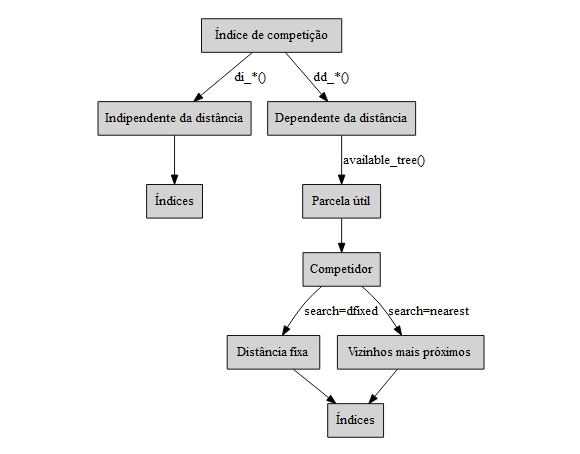
\includegraphics{../workflow.png}
\caption{}
\end{figure}

\subsection{Competition indices}\label{competition-indices}

Foram inplementados difersos indices dependentes e independentes da
distancia. Cada índice, identificado com o nome do autor que o propôs,
tem um função própria e é calculado individualmente. Os índices
independetes da distância necessitam obrigatoriamente do diâmetro das
árvores e eventualmente da área da parcela amostral. Já os índices
dependentes da distância exigem além do diâmetro, as coordenadas das
árvores em um plano cartesiano, seja ele real ou hipotético, e do método
que considera uma árvore vizinha como competidora.

\subsection{selection of competitors}\label{selection-of-competitors}

Para determinar se uma árvore é competidora, é necessário determinar ou
o raio de busca que tem como centro a árvore objeto, ou especificar o
número de árvores mais proximas que serão consideradas como
competidoras. A Figura 1 mostra 25 árvores hipotéticas, dispostas de
maneira regular. A partir da árvore objeto, todas as árvores vizinhas
que estiverem dentro do circulo com raio de 2,5 m são consideradas como
competidoras. A determinação do raio de busca ou do número de arvores
mais próximas é determinada pelo pesquisador e tem impacto relevante no
cálculo dos índices dependentes da distância.

\section{Case study}\label{case-study}



\end{document}

